\section{Bonus Results}

\subsection{Sentence-similarity quality}

\begin{comment}

\begin{table}[]
    \centering
    \begin{tabular}{ccc}
        \toprule
        & EN $\rightarrow$ DE & DE $\rightarrow$ EN \\
        \midrule
        BCN & .579 & .570 \\
        IMG\_PIVOT & .772 & .763 \\
        DPCCA & .826 & .791 \\
        \midrule 
        \emph{align} & .813 & .833 \\
        \emph{align} + c2c & .920 & .906\\
        \bottomrule
    \end{tabular}
    \caption{Results on translation retrieval on the Multi30K translation portion test set.}
    \label{tab:translate}
\end{table}
\end{comment}

\begin{comment}
\begin{table*}[]
    \centering
    \begin{tabular}{llll|lll}
    \toprule
 & & & & EN $\rightarrow$ DE & DE $\rightarrow$ EN \\
 \midrule
         BCN & & & & 57.9 & 57.0 \\
          IMG\_PIVOT & & & &  77.2 & 76.3 \\
         DPCCA & & & &  82.6 & 79.1 \\
    \midrule
        C2C  &En & De & COCO &     \\
        \midrule
        & \checkmark &    \checkmark &   & 81.7   & 80.4  \\
        & \checkmark &    \checkmark & \checkmark  & 82.5    & 81.0    \\
        &  & \checkmark     &   \checkmark &   73.4 &  70.7  \\

        \checkmark    & \checkmark &    \checkmark &   & 90.6   & 91.2  \\
        \checkmark & \checkmark &    \checkmark & \checkmark  & 90.0   & 90.1  \\
        \bottomrule
    \end{tabular}
    \caption{Results on translation retrieval on the Multi30K translation portion validation set. ONLY ONE SEED: 57493}
    \label{tab:translate}
\end{table*}
\end{comment}

\begin{table}[]
    \centering
    \begin{tabular}{lcc}
    \toprule
    & EN $\rightarrow$ DE & DE $\rightarrow$ EN \\
    \midrule
    \citet{rajendran2015bridge} & 57.9 & 57.0 \\
    \citet{gella2017image} &  77.2 & 76.3 \\
    \citet{rotman2018bridging} &  82.6 & 79.1 \\
    \midrule
    En + De & 82.7   & 83.4  \\
    \; + c2c & 90.6   & 91.2  \\
    En + De + COCO & 82.5    & 81.0    \\
    \; + c2c & 90.0   & 90.1  \\
    De + COCO & 73.4 &  70.7  \\
        \bottomrule
    \end{tabular}
    \caption{Results on translation retrieval on the Multi30K translation portion validation set. ONLY ONE SEED: 57493}
    \label{tab:translate}
\end{table}

Here we estimate the capability of our model to identify
translation equivalent caption pairs by utilizing the English-German
translation pairs from M30K. 
These results help us estimate how much 
trust should be attributed to the different models
to generate their own pseudopairs using 
the sentence-similarity strategy.

Furthermore, we are interested how well
do the representations encode translation equivalence even if 
no translation data was provided i.e. models without 
the +c2c loss solely learn the 
relationship between languages through using the images 
as pivots. We then move on to gauge how much these 
results are improved when using
the caption--caption loss. Note that this objective takes pairs
of captions in different languages belonging to the same image
as such it is still a noisy supervision for this task.


In Table~\ref{tab:translate}
we report the R@1 of retrieving the correct translation for 
English sentences given the German caption and vica-versa on 
the translation portion of the test set of M30K.
We compare with the best approaches to our knowledge as
reported by \cite{rotman2018bridging}. 
We report the best best version of their
model (DPCCA), which is a deep partial canonical correlation 
analysis method  maximizing the correlation between
captions of the same image conditioned 
on image representations. The Bridge Correlation Network (BCN) 
\cite{rajendran2015bridge} is also trained to maximize the 
correlation between the sentences using images as pivots.
IMG\_PIVOT \cite{gella2017image} is the most comparable architecture
with the only difference that it uses the VGG-19 
features instead of ResNet, sum-of-hinges instead 
of max-of-hinges loss and no c2c objective. 

Our models seem to improve upon the state-of-the-art currently
held by DPCCA.  We find this results interesting as 
\cite{rajendran2015bridge} note that DPCCA improves over the
CNN+RNN style models even though it is less complex. However,
in our setup the \emph{aligned plus disjoint} (En+De+COCO) model
is on par in performance with the DPCCA even though it is not 
explicitly trained to match sentences.
Adding the c2c loss brings our approach closer to the 
DPCCA in that here we also explicitly push sentences closer 
to each other in the embedding space and find our results
significantly better than that of the
DPCCA approach. 

We find that adding more monolingual English data
in from COCO to the bilingual M30K model improves retrieval
performance. Comparing the aligned bilingual M30K model to the disjoint M30K German and 
English COCO setup we find that disjoint model has a much lower retrieval performance on
this task. This result suggests that the disjoint model generates lower quality pseudo-pairs,
which provides explanation for the worse performance. On the other hand we find a large  
improvement when using the caption--caption loss, which suggests higher quality pseudo-pair 
data for the c2c model, explaining the superior performance.

\subsection{Sum- vs. Max-violation}

%\textbf{Is it better to train an image--sentence model with sum- or max-violation? Faghri does not comprehensively show this because their single-crop results on VGG19 suggest no difference. Most of their best results are with random cropping on ResNet.}

Following \cite{kadar2018conll} in all our experiments we used the max-violation 
objective function -- see Equation~\ref{eq:maxviol} -- , however many architectures apply
the sum-violation -- see Equation~\ref{eq:sumviol} --  in the context of image-sentence 
ranking \cite{nam2017dual} multilingual grounded learning \cite{gella2017image} and 
grounded learning from speech signal \cite{chrupala2017representations}. The article
introducing the max-violation loss function \cite{faghri2017vse++} compares sum- and 
max-violation objectives and do not show improved performance on Flickr30K 
in the setting most similar to
ours: fixed center-crop VGG-19 image features throughout training (as opposed to fine-tuning 
and/or random crops). Here we systematically compare the two loss functions 
in our center-crop 
ResNet50 feature setup in monolingual, bilingual experiments and with the addtional 
caption--caption loss.  The results are shown on Figure~\ref{fig:summax}: each 
value we report is the sum of recall scores R@1, R@5 and R@10
across both T $\rightarrow$ I and I $\rightarrow$ T and both
English and German.
In all conditions we find improvements with the max-violation objective
compared to the sum-violation.

\begin{equation}
\label{eq:sumviol}
\begin{split}
\mathcal{J}(a, b) = \sum_{<\hat{a}, b>}[\text{max}(0, \alpha - s(a,b) + s(\hat{a}, b))] \;+ \\ \sum_{<a, \hat{b}>}[\text{max}(0, \alpha - s(a,b) + s(a, \hat{b}))]
\end{split}
\end{equation}




\begin{figure}
    \centering
    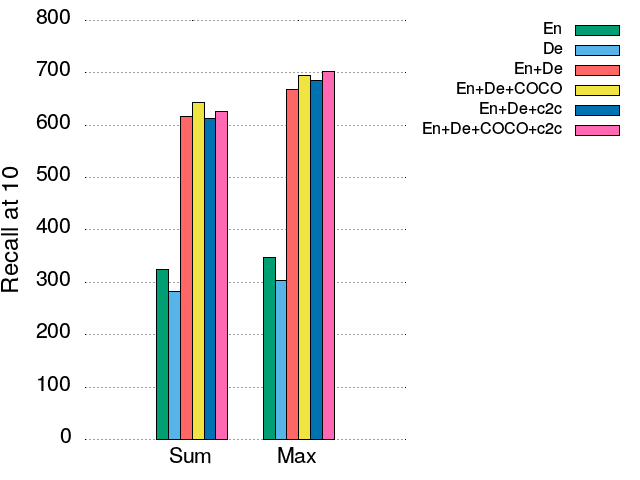
\includegraphics[scale=0.45]{assets/summax.png}
    \caption{Comparing Sum- and Max-violation loss. The reported values are the sum of recall scores 
            across R@1, R@5 and R@10 for both image-to-text and text-to-image retrieval for both English and german.
            Each value is the average of 3 runs.}
    \label{fig:summax}
\end{figure}

\section{Pseudo-pair set characteresitics}
The pseudo-pairs generated by the En+De+COCO model with caption--caption loss are made up of
approximately only 40\% of the German captions available in M30K -- 50000 out of 145000. 
Filtering out the bottom 25\% of sentences results in around 30\%, 
while keeping only the top 25\% results in featuring only 10\% of the 
captions. This means that the same captions are re-used a large number of 
times in the pseudo-pair data set. Taking a look at the frequency distribution of 
the pseudo-captions reveals further that a few sentences are used in most of the data set: 
the 150 most common captions cover approximately 20\%  of the full data set.
The pseudo-pair data set generated by the same model without the caption--caption loss
has very similar characteristics. It uses approximately 39\% of the M30K German captions
and the 150 most common captions also cover 20\% of the pseudo-pair set. However, we find
that the c2c pseudo-pairs cover a larger vocabulary: using the same pre-processing scheme
to compute the vocabulary as in the experiments the average vocabulary-size 
across three random seeds of the 
c2c pseudo-pairs is 12679.3, while without the c2c objective it is only 11657.0. 
The average overlap between the generated pseudo-pairs across all three seeds
for both models with and without c2c is 0.53 (jaccard coefficient). The overlap 
between the the models considering all 6 seed pairs is 0.46.



\begin{comment}
\begin{table*}[]
    \centering
    \begin{tabular}{cccc|cccc}
    \toprule
       & \multicolumn{3}{c}{Sources} & \multicolumn{2}{c}{Max}  & \multicolumn{2}{c}{Sum} \\[1ex]
        C2C& En & De & COCO & En &  De   & En &  De  \\
        \midrule
        & \checkmark & &  & 348.2     & & 324.9 &    \\
        & &    \checkmark &  &   & 303.9  & & 281.9  \\
        & \checkmark &    \checkmark &   & 352.8  & 315.5 & 323.6 & 293.0 \\
        & \checkmark &    \checkmark & \checkmark  & 373.0   & 321.5 & 344.8 & 299.0 \\
     \midrule   
    \checkmark    & \checkmark &    \checkmark &   & 357.9
  & 326.6 & 318.4 & 294.5 \\
   \checkmark     & \checkmark &    \checkmark & \checkmark  & 372.5  & 330.4     & 330.6 & 295.6 \\
        
        \bottomrule
    \end{tabular}
    \caption{Comparing Sum- and Max-violation loss. The reported values are the sum of recall scores 
            across R@1, R@5 and R@10 for both image-to-text and text-to-image retrieval. Each value is the
            average of 3 runs.}
    \label{tab:summax}
\end{table*}
\end{comment}

\begin{comment}


\begin{table}[]

    \centering
    \begin{tabular}{lcc}
    \toprule
    & T $\rightarrow$ I & I $\rightarrow$ T \\
    \midrule
    M30K & 69.8  & 81.6 \\
    COCO & 58.3 & 68.9  \\
    M30K + COCO & \bf{74.4}  &  \bf{84.8}\\
    \bottomrule
    \end{tabular}
    \caption{Seed 409, early stopping done and R@10 reported on the dev set of the M30K datasets.}
    \label{tab:domain}
\end{table}

\end{comment}